En esta sección se describe el diseño del lenguaje junto con su semántica.
Luego se explica de que manera es traducido a un lenguaje de bajo nivel, más
simple de interpretar, el cuál podrá ser interpretado por implementaciones de
una máquina virtual en diferentes plataformas de hardware.

También se describirá las etapas de compilación, desde que se escribe
un programa en alto nivel, hasta que el mismo es ejecutado en una
plataforma objetivo.

El siguiente diagrama resume todas las etapas y componentes necesarios:

\begin{figure}[hbtp]
\begin{center}
\caption{Etapas y componentes}
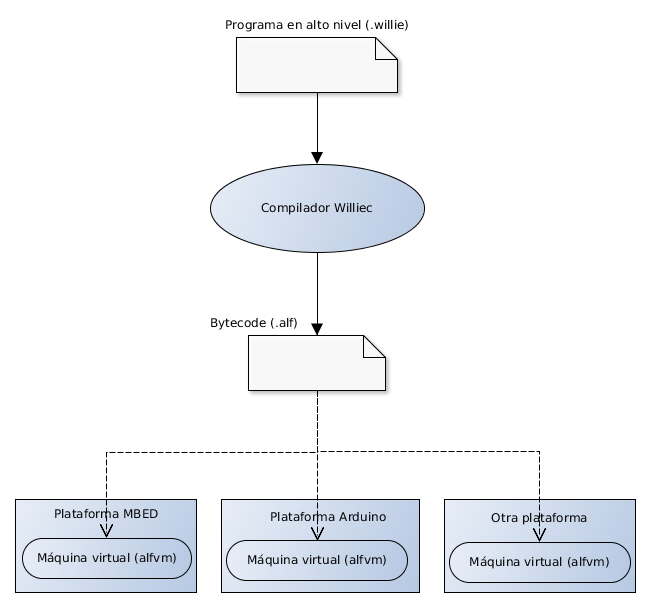
\includegraphics[width=0.9\textwidth]{graphs/compilacion.png}
\label{fig:compilacion}
\end{center}
\end{figure}

\section{Lenguaje de alto nivel}

  Un programa constará de dos secciones principales, una sección de declaraciones, donde
se declararán funciones y una sección donde se aplicarán combinadores de programación
funcional reactiva, especificando cómo son transformadas las señales para especificar
el comportamiento de los robots.

\subsection{Declaraciones}

  Las funciones se declaran de la siguiente manera.

\begin{verbatim}
    nombre argumento_1 .. argumento_n = expresion
\end{verbatim}

  Donde una expresión puede ser un valor,
una expresión aritmética (por ejemplo una suma o multiplicación),
una aplicación de una función, o una expresión condicional.\\

%  La sintaxis es muy similar a la del lenguaje \texttt{Haskell}, aunque
%no se permiten funciones anónimas, y los cálculos se hacen
%inmediatamente (no cuenta con evaluación a demanda \emph{lazy evaluation}).

  Para declarar un valor constante simplemente se escribe:

\begin{verbatim}
    NOMBRE_CONSTANTE = valor
\end{verbatim}

  Ejemplo de declaración:

\begin{verbatim}
    # fibonacci
    fibo n = if (n < 2) then (1) else (fibo(n-1) + fibo(n-2))
\end{verbatim}

\subsection{Combinadores de FRP}

  Las entradas en el robot se puden manipular utilizando la función \texttt{read}.
  La misma crea una señal que cambia de acuerdo a los valores recibidos en la entrada.\\

  Para aplicar una función a una señal, se aplica el combinador \texttt{lift} el cuál toma
  una función y una señal y produce una nueva señal resultado de la aplicación.

  Luego se usa una lista de aplicaciones de \texttt{lift},
\texttt{lift2} y \texttt{folds} para combinar las señales hasta
obtener los valores que conformarán la salida del robot y su estado.\\
  La función \texttt{output} se utiliza para mapear esas señales a las
salidas correspondientes.\\

  La función \texttt{lift} combina una función y un valor
dependiente del tiempo, y crea un nuevo valor dependiente
del tiempo, es decir, aplica una función que transforma
una señal en otra:\\

$lift :: (a \rightarrow b) \rightarrow Signal\ a \rightarrow Signal\ b$\\

  Para combinar señales, se utiliza la función \texttt{lift2}
que recibe dos señales y produce una nueva aplicando una
función.\\

$lift2 :: (a \rightarrow b \rightarrow c) \rightarrow Signal\ a \rightarrow Signal\ b \rightarrow Signal\ c$\\

Utilizando \texttt{lift2} se pueden definir funciones \texttt{liftN}
combinándola suscesivas veces, por ejemplo:\\
\\
$lift3 :: (a \rightarrow b \rightarrow c \rightarrow d) \rightarrow Signal\ a \rightarrow Signal\ b \rightarrow Signal\ c \rightarrow Signal\ d$\\
$lift3\ f\ sa\ sb\ sc = lift2\ ((lift2\ f\ sa\ sb)\ sc)$\\

Para crear señales que no solo dependen de otra señal, sinó que dependen
de ella y además de su historia (los valores anteriores),
se define otro combinador \texttt{folds}
que cuando recibe los valores de la señal, los combina y acumula. Éste
combinador es análogo a la operación \texttt{fold} sobre listas.\\

$folds :: (a \rightarrow b \rightarrow b) \rightarrow b \rightarrow Signal\ a \rightarrow Signal\ b$\\

\subsection{Ejemplo}

  En el siguiente ejemplo se muestra como haría para detener un
robot cuando su sensor de distancia muestra un valor menor a un mínimo.

\begin{verbatim}
INPUT_DISTANCE = 1
OUTPUT_MOTOR = 1

MIN_DISTANCE = 30
FULL_SPEED = 100
STOP = 0

distanceToSpeed n = if (n < MIN_DISTANCE) then STOP else FULL_SPEED

do {
  distance <- read INPUT_DISTANCE,
  speed <- lift distanceToSpeed distance,
  output OUTPUT_MOTOR speed
}

\end{verbatim}

Primero se definió una fuente de eventos llamada \emph{distance},
de tipo \emph{Event Number}.

\begin{verbatim}
  distance <- read INPUT_DISTANCE
\end{verbatim}

La misma emitirá un evento con la distancia en \emph{cm} leída
por un sensor en el robot.

  Luego, se quiere que cuando la distancia sea menor al valor
\emph{MINIMO} dado, el robot se detenga completamente, ésto
quiere decir, que la velocidad sea $0$, en otro caso el mismo
se mueve a velocidad $100$, la cuál asumimos es una velocidad
apropiada.
  Para ésto se crea una nueva fuente de eventos, definida a partir
de \emph{distance}, aplicandole la función \texttt{distanceToSpeed} 
a cada valor para obtener la velocidad.

\begin{verbatim}
  speed <- lift distanceToSpeed distance
\end{verbatim}

  Ésta expresión, también es una fuente de eventos
de tipo \emph{Event Number}.

  Finalmente, se aplica la función nativa \texttt{output} cuyo
primer parámetro es el $id$ de la salida, en éste caso es \texttt{OUTPUT\_MOTOR}
y su segundo parámetro es una fuente de eventos,
en éste caso son velocidades.


\section{Lenguaje de bajo nivel}

  Para presentar el lenguaje, primero defino las estructuras
necesarias para explicar la semántica de cada instrucción.

\begin{enumerate}

\item \emph{Inputs}

  Los valores leídos en las entradas de hardware se mapean
en esta lista. Por ejemplo si el hardware cuenta con un botón,
y el identificador del botón es $i$,
su valor se representará con la notación:

  $Inputs_i$

  A cada entrada se le asocia un conjunto de
rutinas que deben invocarse cuando se tenga un
valor disponible en la entrada. El mismo puede ser vacío si
no hay rutinas esperando por su valor. Queda a criterio de quien
implementa la máquina si éstos valores deben ser guardados o
descartados.
  A éste conjunto de rutinas lo denotamos cómo:

  $Callbacks_i$

\item \emph{Nodes}

  Es utilizado para almacenar todas las transformaciones de señales.
  Cada nodo, tiene una lista de otros nodos que dependen de él y la
  posición del argumento por el que esperan.
  Además el nodo almacena el último valor calculado, y una lista
  de argumentos que le serán pasados, si son nuevos o no.

  Cada aplicación de \texttt{lift}, \texttt{lift2} o \texttt{folds}
será mapeada en un nodo.

  Cada nodo $Node_i$ tiene una lista de nodos adyacentes
que dependen de él.

\item \emph{Outputs}

  Mapea señales en salidas de hardware, los valores
son asignados con la operación \texttt{output}.

\item \emph{Stack}

Es una pila global, se utiliza para ejecutar operaciones,
realizar cálculos, es único
y global, y los hilos de ejecución no pueden guardar valores
persistentes en él.

Usaremos el símbolo $TOS$ para referirnos al elemento en el tope
de la pila y $Stack$ para referirnos a la pila.

\item \emph{Ready}

Es una \emph{cola} que contiene punteros a los nodos
listos para ser ejecutados.

\item \emph{Dispatcher}

El dispatcher, es quien implementa las acciones de la máquina.
El mismo se encarga de recibir valores de los sensores, mapearlos
a eventos en las entradas $Input_i$.

Éstos eventos, serán recibidos por los nodos $Nodes$, cada $Node_i$
que espera por eventos, entrará en estado activo cuando todos los nodos
por los que espera le envíen un evento.
A su vez, el nodo en estado activo calcula un resultado y notifica a
todos sus nodos adyacentes.

El dispatcher, realizará implicitamente un orden topológico de los
nodos, como $Nodes$ es un grafo acíclico, éste proceso es posible y termina, y cada
salida cuenta con un valor, que será mapeado a los actuadores.

\end{enumerate}

\subsection{Instrucciones}

  A continuación se listan las instrucciones de bajo nivel
  más relevantes junto con su semántica.

\begin{itemize}
\item \texttt{lift id source\_id function\_pointer}

 Crea un nodo que recibe valores de la fuente de
 eventos $source_id$,
 les aplica la función $function_pointer$ y emite el resultado
 en la fuente de eventos $id$.\\
 El nodo se agrega a $Nodes$ y el dispatcher se encargará de aplicar
 la función siempre que sea necesario.

\item \texttt{lift2 id source-id\_1 source-id\_2 function\_pointer}

 Crea un nodo que recibe valores de $source-id_1$ y
 $source-id_2$,
 les aplica la función $function_pointer$ y emite el resultado
 en la fuente de eventos $id$.\\
 Cuando reciba un valor nuevo por cada uno de los que espera, el
 dispatcher aplica la función y emite el resultado.

\item \texttt{read id input-id}

 Agrega un nodo a $Nodes$ que recibe valores de una entrada,
 y emite el resultado en la fuente de eventos $id$.
 Cuando el dispatcher reciba un cambio en la entrada, el nodo emitirá
 el resultado.

\item \texttt{write index id}

  Crea un nodo $Output$ que recibe valores de la señal $id$
  y los emite en la salida número $index$.
  El nodo guarda dicho valor y el dispatcher decide en que momento
  debe escribirlo en la salida asociada.
  Se intentará que sea lo más instantáneo posible
  ya que el valor depende del tiempo y a mayor demora, menos correcto
  será el comportamiento.

\end{itemize}

\pagebreak
\section{Compilador}

  El compilador será el encargado de leer el programa de alto nivel y
traducirlo al lenguaje de bajo nivel.

  El programa resultado tendrá al principio las traducción de las instrucciones
correspondientes al bloque \texttt{do}. Las mismas al ser ejecutadas armarán el
grafo de señales del programa.\\
  Al final del bloque, habrá una instrucción \texttt{halt} que cederá el control
al $dispatcher$.\\
  Luego estará el código correspondiente a cada función definida. Cada invocación
a función, tendrá la referencia directa hacia la posición en el código de la misma.

  El compilador constará de dos etapas principales.

  En la primer etapa lee el programa de alto nivel y
  genera un árbol de sintaxis
  abstracto (AST) del mismo. Dicha etapa es llamada análisis sintáctico.\\

  Luego el ast se recorre y la segunda etapa es la generación del
  código de bajo nivel.\\

  En la siguiente figura se puede ver la estructura más detallada
  del compilador.

\begin{figure}[hp]
\begin{center}
\caption{Diagrama del compilador}
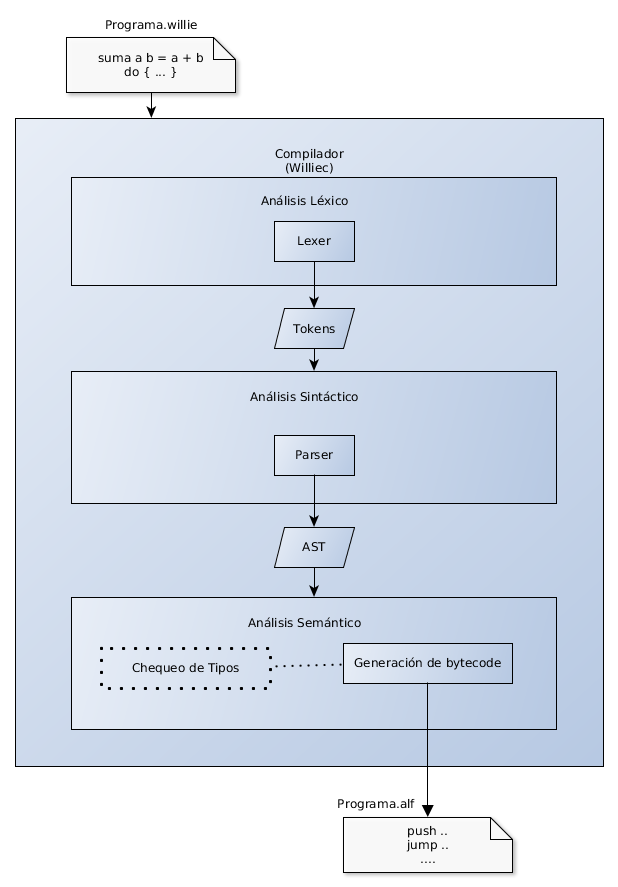
\includegraphics[width=0.9\textwidth]{graphs/compiler.png}
\label{fig:compiler}
\end{center}
\end{figure}

\newpage
\subsection{Ejemplo de traducción}

Dado el siguiente programa de ejemplo en alto nivel:

\begin{verbatim}
# Este programa de prueba muestra con un led si se esta frente a una casa.

#Inputs
sensor_distancia = 1
#Outputs
led = 1

hay_casa = \distancia -> (distancia < 100)

do {
  signal_distancia = read sensor_distancia,
  signal_viendo = lift hay_casa sensor_distancia,
  write led signal_viendo
}
\end{verbatim}

El mismo se representaría en bajo nivel de la siguiente forma:

\begin{verbatim}
01:  push 1
02:  store 0 //sensor_distancia = 1
03:  push 1
04:  store 1 //led = 1
05:  read 0 0 //signal_distancia = read 0
06:  lift 1 0 hay_casa //signal_viendo = lift hay_casa sensor_distancia
07:  write 1 1 //write led signal_viendo
08:  halt
09:  load_arg 0 //hay_casa:
10:  push 100
11:  cmp_le //distancia < 100
12:  return
\end{verbatim}

\section{Máquina Virtual}

  La máquina virtual será la encargada de recibir el bytecode creado por
el compilador, e interpretarlo en la plataforma que esté ejecutando.
  A diferencia del compilador, es necesario implementar una máquina virtual
para cada arquitectura objetivo.\\

  Por ejemplo, para ejecutar programas en un robot
  con un procesador \emph{arduino}, debe
  existir una implementación de la máquina para ese modelo
  de \emph{arduino}.

  Al momento de implementar la máquina, se tomará en cuenta ésto para
  factorizar partes en común y sólo implementar por arquitectura, las
  partes que realmente sean diferentes como ser la comunicación con
  los periféricos de entrada/salida y las llamadas al sistema.

